\documentclass{beamer}
\usepackage{amsmath}
\usepackage{hyperref}
\usepackage{listings}
\usepackage{xcolor}
\hypersetup{colorlinks=true, citecolor=blue, filecolor=blue, linkcolor=blue, urlcolor=blue}
\definecolor{codegreen}{rgb}{0,0.6,0}
\definecolor{codegray}{rgb}{0.5,0.5,0.5}
\definecolor{codepurple}{rgb}{0.58,0,0.82}
\definecolor{backcolour}{rgb}{0.95,0.95,0.92}
 
\lstdefinestyle{mystyle}{
    backgroundcolor=\color{backcolour},   
    commentstyle=\color{codegreen},
    keywordstyle=\color{magenta},
    numberstyle=\tiny\color{codegray},
    stringstyle=\color{codepurple},
    basicstyle=\ttfamily\footnotesize,
    breakatwhitespace=false,         
    breaklines=true,                 
    captionpos=b,                    
    keepspaces=true,                 
    %numbers=left,                    
    numbersep=5pt,                  
    showspaces=false,                
    showstringspaces=false,
    showtabs=false,                  
    tabsize=2
}
 
%%
%% Julia definition (c) 2014 Jubobs
%%
\lstdefinelanguage{Julia}%
  {morekeywords={abstract,break,case,catch,const,continue,do,else,elseif,%
      end,export,false,for,function,immutable,import,importall,if,in,%
      macro,module,otherwise,quote,return,switch,true,try,type,typealias,%
      using,while},%
   sensitive=true,%
   alsoother={$},%
   morecomment=[l]\#,%
   morecomment=[n]{\#=}{=\#},%
   morestring=[s]{"}{"},%
   morestring=[m]{'}{'},%
}[keywords,comments,strings]%

\lstset{%
    language         = Julia,
    basicstyle       = \ttfamily,
    keywordstyle     = \bfseries\color{blue},
    stringstyle      = \color{magenta},
    commentstyle     = \color{ForestGreen},
    showstringspaces = false,
}
 
 
\lstset{style=mystyle}

\mode<presentation> {

% The Beamer class comes with a number of default slide themes
% which change the colors and layouts of slides. Below this is a list
% of all the themes, uncomment each in turn to see what they look like.

%\usetheme{default}
\usetheme{AnnArbor}
%\usetheme{Antibes}
%\usetheme{Bergen}
%\usetheme{Berkeley}
%\usetheme{Berlin}
%\usetheme{Boadilla}
%\usetheme{CambridgeUS}
%\usetheme{Copenhagen}
%\usetheme{Darmstadt}
%\usetheme{Dresden}
%\usetheme{Frankfurt}
%\usetheme{Goettingen}
%\usetheme{Hannover}
%\usetheme{Ilmenau}
%\usetheme{JuanLesPins}
%\usetheme{Luebeck}
%\usetheme{Madrid}
%\usetheme{Malmoe}
%\usetheme{Marburg}
%\usetheme{Montpellier}
%\usetheme{PaloAlto}
%\usetheme{Pittsburgh}
%\usetheme{Rochester}
%\usetheme{Singapore}
%\usetheme{Szeged}
%\usetheme{Warsaw}

% As well as themes, the Beamer class has a number of color themes
% for any slide theme. Uncomment each of these in turn to see how it
% changes the colors of your current slide theme.

%\usecolortheme{albatross}
%\usecolortheme{beaver}
%\usecolortheme{beetle}
%\usecolortheme{crane}
%\usecolortheme{dolphin}
%\usecolortheme{dove}
%\usecolortheme{fly}
%\usecolortheme{lily}
%\usecolortheme{orchid}
%\usecolortheme{rose}
%\usecolortheme{seagull}
%\usecolortheme{seahorse}
%\usecolortheme{whale}
%\usecolortheme{wolverine}

%\setbeamertemplate{footline} % To remove the footer line in all slides uncomment this line
\setbeamertemplate{footline}[page number] % To replace the footer line in all slides with a simple slide count uncomment this line

\setbeamertemplate{navigation symbols}{} % To remove the navigation symbols from the bottom of all slides uncomment this line
}

\usepackage{graphicx} % Allows including images
\usepackage{booktabs} % Allows the use of \toprule, \midrule and \bottomrule in tables
%\usepackage {tikz}
\usepackage{tkz-graph}
\GraphInit[vstyle = Shade]
\tikzset{
  LabelStyle/.style = { rectangle, rounded corners, draw,
                        minimum width = 2em, fill = yellow!50,
                        text = red, font = \bfseries },
  VertexStyle/.append style = { inner sep=5pt,
                                font = \normalsize\bfseries},
  EdgeStyle/.append style = {->, bend left} }
\usetikzlibrary {positioning}
%\usepackage {xcolor}
\definecolor {processblue}{cmyk}{0.96,0,0,0}
%----------------------------------------------------------------------------------------
%	TITLE PAGE
%----------------------------------------------------------------------------------------

\title[Trust Region Methods]{Numerical Optimization: Trust Region Methods} % The short title appears at the bottom of every slide, the full title is only on the title page

\author{Qiang Zhu} % Your name
\institute[University of Nevada Las Vegas] % Your institution as it will appear on the bottom of every slide, may be shorthand to save space
{
University of Nevada Las Vegas\\ % Your institution for the title page
\medskip
}
\date{\today} % Date, can be changed to a custom date

\begin{document}

\begin{frame}
\titlepage % Print the title page as the first slide
\end{frame}

\begin{frame}
\frametitle{Overview} % Table of contents slide, comment this block out to remove it
\tableofcontents % Throughout your presentation, if you choose to use \section{} and \subsection{} commands, these will automatically be printed on this slide as an overview of your presentation
\end{frame}

%----------------------------------------------------------------------------------------
%	PRESENTATION SLIDES
%----------------------------------------------------------------------------------------

%------------------------------------------------

\section{Trust Region Model}
\begin{frame}{The problem of line search}
In the line search method, one usually use the direction based on the first- or second-order derivative, and then do an approximate 1D search. 
If the derivative is far from the local minimum, such search may result in excessively large steps or premature convergence.

\begin{figure}
\centering
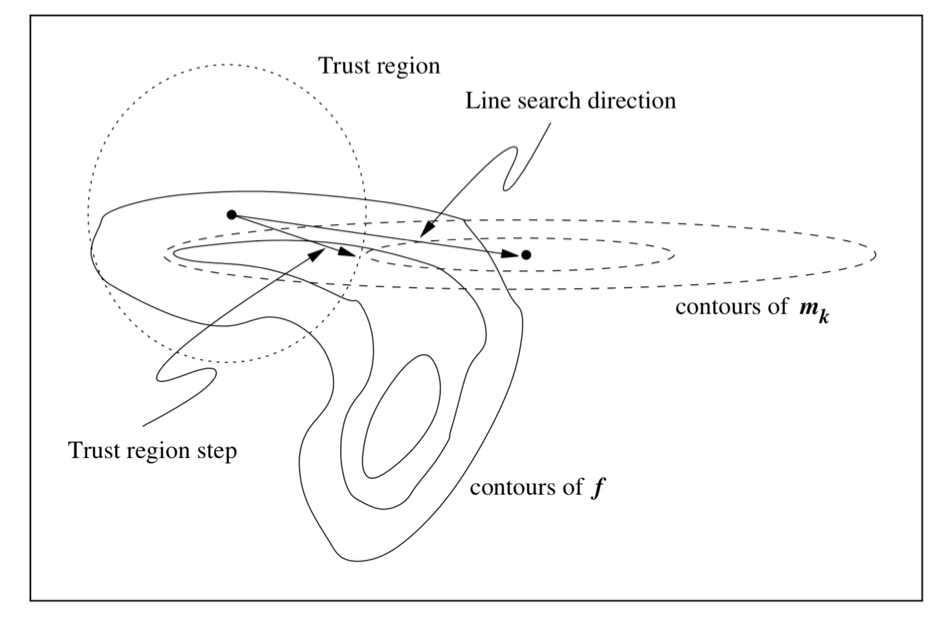
\includegraphics[width=90mm]{Lecture_notes/Figs/trust-region.jpeg}
\end{figure}
\end{frame}

\begin{frame}{Line search .v.s trust region}
\begin{alertblock}{Line search}
\begin{itemize}
    \item Find the direction of improvement
    \item Select a step length
\end{itemize}
\end{alertblock}
\vfill
\begin{alertblock}{Trust region}
\begin{itemize}
    \item Select a trust region (within a hypersphere)
    \item Find a point of improvement
\end{itemize}
\end{alertblock}

\end{frame}

\section{The outline of trust region approach}
\begin{frame}{Quadratic approximation}
In this chapter, we will assume that the model function $m_k$ that is used at each iterate $x_k$ is quadratic. 
$m_k$ is based on the Taylor-series expansion of $f$.
\begin{equation*}
    f(x_k + p) = f(x_k) + \nabla f(x_k)^T p + \frac{1}{2}p^T \nabla^2 f(x_k + tp)p,
\end{equation*}
where $t$ is some scalar in the interval (0,1). 

By using an approximation $B_k$ to the Hessian in the second-order term, $m_k$ is defined as follows:
\begin{equation*}
    m_k(p) = f(x_k) + \nabla f(x_k)^T p + \frac{1}{2}p^T B_k f(x_k + tp)p,,
\end{equation*}

The difference between $m_k(p)$ and $f(x_k + p)$ is $O(p^2)$ ,which is small when $p$ is small.

\end{frame}

\begin{frame}{Trust region step}
The trust-region method steps to the minimizer of $m_k$ within the dotted circle, yielding a more significant reduction in $f$ and better progress toward the solution.

To obtain each step, we seek a solution of the subproblem
\begin{gather*}
    \textrm{min}~ m_k(p) = f(x_k) + \nabla f(x_k)^T p + \frac{1}{2}p^T B_k f(x_k + tp)p, \\
    \textrm{s.t.}~~ ||p||_2 \leq \Delta_k,    
\end{gather*}

where $\Delta_k$ is the \textcolor{blue}{trust-region radius}.

Thus, the trust-region approach requires us to solve a sequence of subproblems
in which the objective function and constraint (which can be written as $p^Tp \leq \Delta_k$)
are both quadratic, which is easy to solve if it is convex. 
\end{frame}

\begin{frame}{How to adjust the $\Delta_k$?}
For a given step, we define 
\begin{equation*}
    \rho_k = \frac{f(x_k) - f(x_k+p_k)}{m_k(0) - m_k(p_k)}
\end{equation*}
The numerator is called the \textcolor{blue}{actual reduction}. \\
The denominator is the \textcolor{blue}{predicted reduction}, which is non-negative. \\

\begin{itemize}
    \item if $\rho_k < 0$, the new objective value $f(x_k + p_k)$ is greater than $f(x_k)$, \textcolor{red}{reject}.
    \item if $\rho_k \approx 1$, there is good agreement between the model $m_k$ and the function $f$, \textcolor{red}{expand the trust region} 
    \item if $0<\rho_k \ll 1$, \textcolor{red}{shrink the trust region} by reducing $\delta_k$
\end{itemize}
\end{frame}

\begin{frame}{Algorithm}

\lstinputlisting[language=julia]{trust.jl}

\end{frame}

\section{Summary}
\begin{frame}{Summary}
    \begin{itemize}
        \item Trust region method may perform better when the initial point is far from the local minimum
        \item The correctness of trust region method relies on the accuracy of the model function
        \item The step size is controled by the trust-region radius which is updated each step
        \item Quadratic approximation needs the information of hessian
        \item The subproblem optimization may be tricky when hessian is not positive definite
    \end{itemize}
\end{frame}
\end{document}

